\documentclass[aspectratio=169]{beamer}
\usefonttheme{professionalfonts}
\usepackage{amsmath,amssymb}
\usepackage{booktabs}
\usepackage{tikz}
\usetikzlibrary{arrows.meta, positioning, calc, decorations.pathmorphing}

\definecolor{myRed}{RGB}{209,34,57}
\definecolor{myBlue}{RGB}{28,90,160}
\definecolor{myGreen}{RGB}{34,139,34}
\definecolor{myOrange}{RGB}{210,105,15}
\definecolor{opRegion}{RGB}{224,244,246}
\definecolor{statorIron}{RGB}{234,240,248}
\definecolor{rotorIron}{RGB}{246,247,250}
\definecolor{airGapCol}{RGB}{255,255,255}
\definecolor{fluxCol}{RGB}{22,82,158}
\definecolor{slotColor}{RGB}{248,242,235}

\title{Comparison: Original vs New TikZ Figures}
\subtitle{ELEC0447 - Synchronous Generators Lecture (Slides 4, 5, 8, 9, 10)}
\author{Antigravity Assistant}
\date{\today}

\begin{document}

\begin{frame}
  \titlepage
\end{frame}

% ----------------------------------------------------
% Slide 4 Comparison
% ----------------------------------------------------
\begin{frame}{Slide 4: Magnetic field created by the stator}
  \begin{columns}[c]
    \begin{column}{0.48\textwidth}
      \centering
      \textbf{\textcolor{black!70}{Original Picture (Raster)}}\\[4pt]
      \fbox{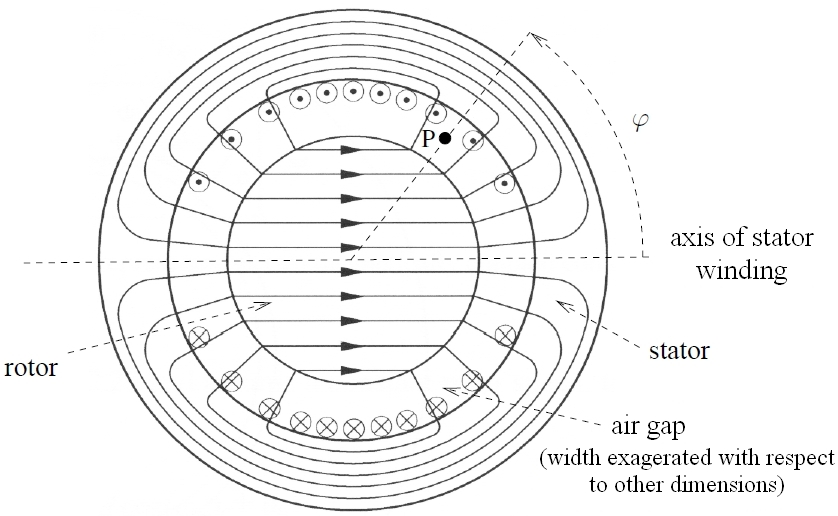
\includegraphics[width=0.92\linewidth,height=0.62\textheight,keepaspectratio]{images/stator_field.jpg}}
    \end{column}
    \begin{column}{0.48\textwidth}
      \centering
      \textbf{\textcolor{myBlue}{New TikZ Figure (Vector)}}\\[4pt]
      \resizebox{0.92\linewidth}{!}{\providecolor{myRed}{RGB}{209,34,57}
\providecolor{myBlue}{RGB}{28,90,160}
\providecolor{myGreen}{RGB}{34,139,34}
\providecolor{myOrange}{RGB}{210,105,15}
\providecolor{statorIron}{RGB}{234,240,248}
\providecolor{rotorIron}{RGB}{246,247,250}
\providecolor{airGapCol}{RGB}{255,255,255}
\providecolor{fluxCol}{RGB}{20,80,165}
\providecolor{slotColor}{RGB}{248,242,235}

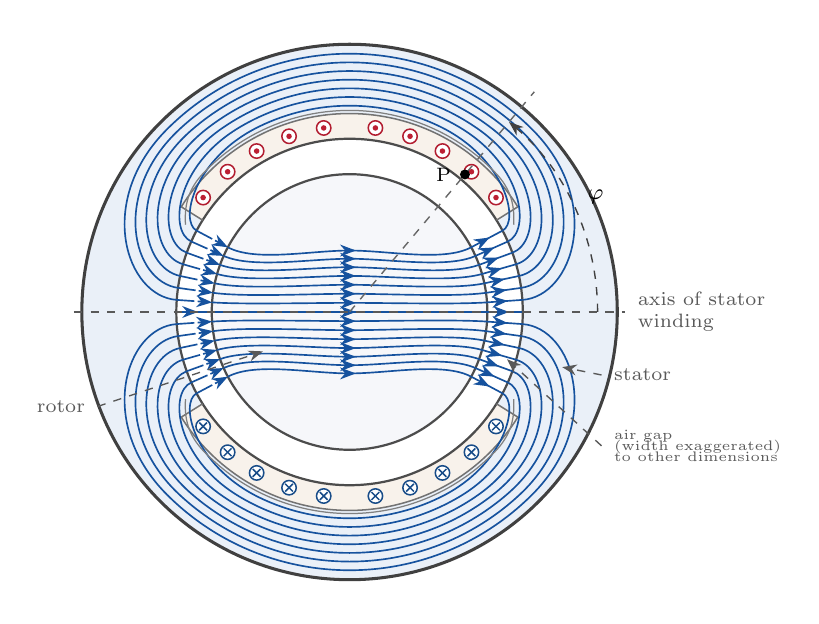
\begin{tikzpicture}[scale=1, >=Stealth, font=\small]

  % Geometry parameters
  \def\Rrotor{1.75}
  \def\Rgap{2.20}
  \def\Rstator{3.40}

  % 1. Iron Cores
  \fill[statorIron] (0,0) circle (\Rstator);
  \fill[airGapCol] (0,0) circle (\Rgap);
  \fill[rotorIron] (0,0) circle (\Rrotor);

  % Slot regions shading
  \fill[slotColor] (32:\Rgap) arc[start angle=32, end angle=148, radius=\Rgap] 
    -- (148:\Rgap+0.32) arc[start angle=148, end angle=32, radius=\Rgap+0.32] -- cycle;
  \fill[slotColor] (-32:\Rgap) arc[start angle=-32, end angle=-148, radius=\Rgap] 
    -- (-148:\Rgap+0.32) arc[start angle=-148, end angle=-32, radius=\Rgap+0.32] -- cycle;

  % Boundaries
  \draw[line width=1.1pt, black!75] (0,0) circle (\Rstator);
  \draw[line width=0.8pt, black!70] (0,0) circle (\Rgap);
  \draw[line width=0.8pt, black!70] (0,0) circle (\Rrotor);

  % Slot outlines
  \draw[line width=0.55pt, black!55] (32:\Rgap) -- (32:\Rgap+0.32) arc[start angle=32, end angle=148, radius=\Rgap+0.32] -- (148:\Rgap);
  \draw[line width=0.55pt, black!55] (-32:\Rgap) -- (-32:\Rgap+0.32) arc[start angle=-32, end angle=-148, radius=\Rgap+0.32] -- (-148:\Rgap);

  % 2. Magnetic Flux Lines
  % Center line along axis
  \draw[line width=0.6pt, fluxCol] (-\Rgap, 0) -- (\Rgap, 0);
  \draw[line width=0.6pt, fluxCol, ->] (0, 0) -- (0.08, 0);
  \draw[line width=0.6pt, fluxCol, ->] (\Rrotor, 0) -- ({(\Rrotor+\Rgap)/2 + 0.05}, 0);
  \draw[line width=0.6pt, fluxCol, ->] (-\Rgap, 0) -- ({-(\Rrotor+\Rgap)/2 + 0.05}, 0);

  % 7 nested symmetrical pairs covering the full depth of the stator yoke
  % dAng: air gap angle. Ri: yoke radius. phiArc: angle where circular arc starts
  \foreach \dAng/\Ri/\phiArc in {
    4/3.28/45,
    8/3.17/47,
    12/3.06/49,
    16/2.95/52,
    20/2.84/55,
    24/2.73/59,
    28/2.62/64
  } {
    \coordinate (RentryR) at (\dAng:\Rrotor);
    \coordinate (RgapR)   at (\dAng:\Rgap);
    \coordinate (RentryL) at ({180-\dAng}:\Rrotor);
    \coordinate (RgapL)   at ({180-\dAng}:\Rgap);

    % Upper half (y > 0)
    % A. Radial segment across air gap with arrow (strictly perpendicular to iron surface)
    \draw[line width=0.6pt, fluxCol, ->] (RentryR) -- (\dAng:{(\Rrotor+\Rgap)/2 + 0.04});
    \draw[line width=0.6pt, fluxCol] (\dAng:{(\Rrotor+\Rgap)/2}) -- (RgapR);

    \draw[line width=0.6pt, fluxCol, <-] (RentryL) -- ({180-\dAng}:{(\Rrotor+\Rgap)/2 - 0.04});
    \draw[line width=0.6pt, fluxCol] ({180-\dAng}:{(\Rrotor+\Rgap)/2}) -- (RgapL);

    % B. Inside rotor: smooth horizontal transition tangent to radial at boundary
    \pgfmathsetmacro{\yMid}{\Rrotor * sin(\dAng) * 0.95}
    \draw[line width=0.6pt, fluxCol]
      (RentryL) .. controls ($(RentryL) + ({-\dAng}:0.4)$) and (-0.5, \yMid) .. (0, \yMid)
      .. controls (0.5, \yMid) and ($(RentryR) + ({180+\dAng}:0.4)$) .. (RentryR);
    \draw[line width=0.6pt, fluxCol, ->] (-0.05, \yMid) -- (0.08, \yMid);

    % C. Stator yoke: fillet from radial at Rgap to azimuthal at Ri, true circular arc across top, and fillet back
    \coordinate (ArcStartU) at (\phiArc:\Ri);
    \coordinate (ArcEndU)   at ({180-\phiArc}:\Ri);
    \pgfmathsetmacro{\filletL}{(\Ri - \Rgap) * 0.6}
    \pgfmathsetmacro{\filletT}{\Ri * sin(\phiArc - \dAng) * 0.6}

    \draw[line width=0.6pt, fluxCol]
      (RgapR) .. controls ($(RgapR) + (\dAng:\filletL)$) and ($(ArcStartU) + ({\phiArc-90}:\filletT)$) .. (ArcStartU)
      arc[start angle=\phiArc, end angle={180-\phiArc}, radius=\Ri]
      .. controls ($(ArcEndU) + ({180-\phiArc+90}:\filletT)$) and ($(RgapL) + ({180-\dAng}:\filletL)$) .. (RgapL);

    % Lower half (y < 0)
    \coordinate (RentryRL) at (-\dAng:\Rrotor);
    \coordinate (RgapRL)   at (-\dAng:\Rgap);
    \coordinate (RentryLL) at ({-180+\dAng}:\Rrotor);
    \coordinate (RgapLL)   at ({-180+\dAng}:\Rgap);

    \draw[line width=0.6pt, fluxCol, ->] (RentryRL) -- (-\dAng:{(\Rrotor+\Rgap)/2 + 0.04});
    \draw[line width=0.6pt, fluxCol] (-\dAng:{(\Rrotor+\Rgap)/2}) -- (RgapRL);

    \draw[line width=0.6pt, fluxCol, <-] (RentryLL) -- ({-180+\dAng}:{(\Rrotor+\Rgap)/2 - 0.04});
    \draw[line width=0.6pt, fluxCol] ({-180+\dAng}:{(\Rrotor+\Rgap)/2}) -- (RgapLL);

    \draw[line width=0.6pt, fluxCol]
      (RentryLL) .. controls ($(RentryLL) + (\dAng:0.4)$) and (-0.5, -\yMid) .. (0, -\yMid)
      .. controls (0.5, -\yMid) and ($(RentryRL) + ({-180-\dAng}:0.4)$) .. (RentryRL);
    \draw[line width=0.6pt, fluxCol, ->] (-0.05, -\yMid) -- (0.08, -\yMid);

    \coordinate (ArcStartL) at (-\phiArc:\Ri);
    \coordinate (ArcEndL)   at ({-180+\phiArc}:\Ri);

    \draw[line width=0.6pt, fluxCol]
      (RgapRL) .. controls ($(RgapRL) + (-\dAng:\filletL)$) and ($(ArcStartL) + ({-\phiArc+90}:\filletT)$) .. (ArcStartL)
      arc[start angle=-\phiArc, end angle={-180+\phiArc}, radius=\Ri]
      .. controls ($(ArcEndL) + ({-180+\phiArc-90}:\filletT)$) and ($(RgapLL) + ({-180+\dAng}:\filletL)$) .. (RgapLL);
  }

  % 3. Conductors in stator slots
  \foreach \a in {38, 49, 60, 71, 82, 98, 109, 120, 131, 142} {
    \coordinate (C) at (\a:{\Rgap+0.16});
    \fill[white] (C) circle (2.6pt);
    \draw[line width=0.55pt, myRed!85!black] (C) circle (2.6pt);
    \fill[myRed!90!black] (C) circle (1.0pt);
  }
  \foreach \a in {-38, -49, -60, -71, -82, -98, -109, -120, -131, -142} {
    \coordinate (C) at (\a:{\Rgap+0.16});
    \fill[white] (C) circle (2.6pt);
    \draw[line width=0.55pt, myBlue!85!black] (C) circle (2.6pt);
    \draw[line width=0.55pt, myBlue!85!black] ($(C)+(-1.4pt,-1.4pt)$) -- ($(C)+(1.4pt,1.4pt)$);
    \draw[line width=0.55pt, myBlue!85!black] ($(C)+(-1.4pt,1.4pt)$) -- ($(C)+(1.4pt,-1.4pt)$);
  }

  % Winding schematic end-turn outline
  \draw[line width=0.45pt, black!50] (28:\Rgap+0.16) [bend right=25] to (45:\Rgap+0.36) arc[start angle=45, end angle=135, radius=\Rgap+0.36] [bend right=25] to (152:\Rgap+0.16);
  \draw[line width=0.45pt, black!50] (-28:\Rgap+0.16) [bend left=25] to (-45:\Rgap+0.36) arc[start angle=-45, end angle=-135, radius=\Rgap+0.36] [bend left=25] to (-152:\Rgap+0.16);

  % 4. Winding Axis
  \draw[dashed, line width=0.55pt, black!65] (-3.5, 0) -- (3.5, 0) 
    node[right=1pt, font=\scriptsize, align=left] {axis of stator\\winding};

  % Point P at angle 50 deg
  \draw[dashed, line width=0.5pt, black!60] (0,0) -- (50:3.65);
  \fill[black] (50:{\Rgap+0.08}) circle (1.8pt) node[left=1.5pt, font=\scriptsize] {P};

  % Angle phi arc
  \draw[->, line width=0.5pt, dashed, black!75] (0:3.15) arc[start angle=0, end angle=50, radius=3.15];
  \node[font=\footnotesize] at (25:3.45) {$\varphi$};

  % 5. Annotations
  \draw[dashed, line width=0.5pt, black!65, ->] (-3.2, -1.2) node[left=1pt, font=\scriptsize] {rotor} -- (-1.1, -0.5);
  \draw[dashed, line width=0.5pt, black!65, ->] (3.2, -1.7) node[right=1pt, font=\tiny, align=left] {air gap\\[-2pt](width exaggerated)\\[-2pt]to other dimensions} -- (2.0, -0.6);
  \draw[dashed, line width=0.5pt, black!65, ->] (3.2, -0.8) node[right=1pt, font=\scriptsize] {stator} -- (2.7, -0.7);

\end{tikzpicture}
}
    \end{column}
  \end{columns}
\end{frame}

% ----------------------------------------------------
% Slide 5 Comparison
% ----------------------------------------------------
\begin{frame}{Slide 5: Three-phase stator winding layout}
  \begin{columns}[c]
    \begin{column}{0.48\textwidth}
      \centering
      \textbf{\textcolor{black!70}{Original Picture (Raster)}}\\[4pt]
      \fbox{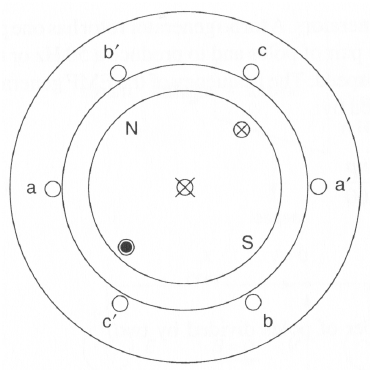
\includegraphics[width=0.92\linewidth,height=0.62\textheight,keepaspectratio]{images/layout_phases.jpg}}
    \end{column}
    \begin{column}{0.48\textwidth}
      \centering
      \textbf{\textcolor{myBlue}{New TikZ Figure (Vector)}}\\[4pt]
      \resizebox{0.88\linewidth}{!}{\providecolor{myRed}{RGB}{209,34,57}
\providecolor{myBlue}{RGB}{28,90,160}
\providecolor{myGreen}{RGB}{34,139,34}
\providecolor{myOrange}{RGB}{210,105,15}
\providecolor{statorIron}{RGB}{234,240,248}
\providecolor{rotorIron}{RGB}{246,247,250}
\providecolor{airGapCol}{RGB}{255,255,255}

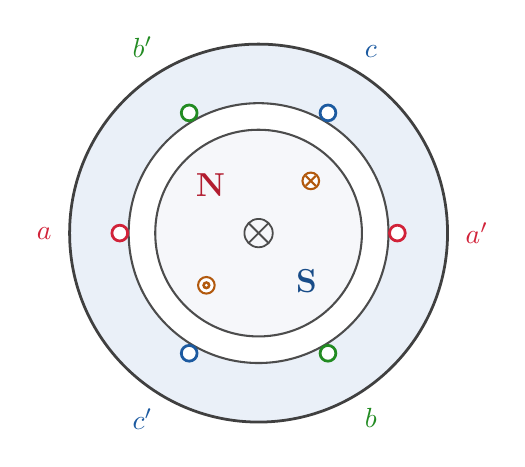
\begin{tikzpicture}[scale=0.75, >=Stealth, font=\small]

  % Radii
  \def\Rrotor{1.75}
  \def\Rgap{2.20}
  \def\Rstator{3.20}

  % 1. Iron Cores
  % Stator core
  \fill[statorIron] (0,0) circle (\Rstator);
  \fill[airGapCol] (0,0) circle (\Rgap);
  
  % Rotor core
  \fill[rotorIron] (0,0) circle (\Rrotor);

  % Boundaries
  \draw[line width=1.0pt, black!75] (0,0) circle (\Rstator);
  \draw[line width=0.75pt, black!70] (0,0) circle (\Rgap);
  \draw[line width=0.75pt, black!70] (0,0) circle (\Rrotor);

  % 2. Central Shaft
  \draw[line width=0.65pt, black!70] (0,0) circle (0.24);
  \draw[line width=0.65pt, black!70] (-0.17,-0.17) -- (0.17,0.17);
  \draw[line width=0.65pt, black!70] (-0.17,0.17) -- (0.17,-0.17);

  % 3. Stator 3-Phase Conductors (single turn: go & return)
  % Phase a (Red): a at 180 deg, a' at 0 deg
  \coordinate (Sa) at (180:{\Rgap+0.15});
  \fill[white] (Sa) circle (3.8pt);
  \draw[line width=1.0pt, myRed] (Sa) circle (3.8pt);
  \node[left=3pt, font=\normalsize\bfseries, text=myRed] at (180:\Rstator) {$a$};

  \coordinate (Saprime) at (0:{\Rgap+0.15});
  \fill[white] (Saprime) circle (3.8pt);
  \draw[line width=1.0pt, myRed] (Saprime) circle (3.8pt);
  \node[right=3pt, font=\normalsize\bfseries, text=myRed] at (0:\Rstator) {$a'$};

  % Phase b (Green): b at 300 deg (-60), b' at 120 deg
  \coordinate (Sb) at (300:{\Rgap+0.15});
  \fill[white] (Sb) circle (3.8pt);
  \draw[line width=1.0pt, myGreen] (Sb) circle (3.8pt);
  \node[below right=1pt, font=\normalsize\bfseries, text=myGreen] at (300:\Rstator) {$b$};

  \coordinate (Sbprime) at (120:{\Rgap+0.15});
  \fill[white] (Sbprime) circle (3.8pt);
  \draw[line width=1.0pt, myGreen] (Sbprime) circle (3.8pt);
  \node[above left=1pt, font=\normalsize\bfseries, text=myGreen] at (120:\Rstator) {$b'$};

  % Phase c (Blue): c at 60 deg, c' at 240 deg
  \coordinate (Sc) at (60:{\Rgap+0.15});
  \fill[white] (Sc) circle (3.8pt);
  \draw[line width=1.0pt, myBlue] (Sc) circle (3.8pt);
  \node[above right=1pt, font=\normalsize\bfseries, text=myBlue] at (60:\Rstator) {$c$};

  \coordinate (Scprime) at (240:{\Rgap+0.15});
  \fill[white] (Scprime) circle (3.8pt);
  \draw[line width=1.0pt, myBlue] (Scprime) circle (3.8pt);
  \node[below left=1pt, font=\normalsize\bfseries, text=myBlue] at (240:\Rstator) {$c'$};

  % 4. Rotor Field Winding Conductors (Orange/Copper)
  % Cross at 45 deg (into page)
  \coordinate (Rf_cross) at (45:1.25);
  \fill[white] (Rf_cross) circle (4.0pt);
  \draw[line width=0.75pt, myOrange!85!black] (Rf_cross) circle (4.0pt);
  \draw[line width=0.75pt, myOrange!85!black] ($(Rf_cross)+(-2.4pt,-2.4pt)$) -- ($(Rf_cross)+(2.4pt,2.4pt)$);
  \draw[line width=0.75pt, myOrange!85!black] ($(Rf_cross)+(-2.4pt,2.4pt)$) -- ($(Rf_cross)+(2.4pt,-2.4pt)$);

  % Dot at 225 deg (out of page)
  \coordinate (Rf_dot) at (225:1.25);
  \fill[white] (Rf_dot) circle (4.0pt);
  \draw[line width=0.75pt, myOrange!85!black] (Rf_dot) circle (4.0pt);
  \fill[myOrange!85!black] (Rf_dot) circle (2.0pt);
  \fill[white] (Rf_dot) circle (0.7pt);

  % 5. Rotor Pole Labels
  \node[font=\large\bfseries, text=myRed!85!black] at (135:1.15) {N};
  \node[font=\large\bfseries, text=myBlue!85!black] at (315:1.15) {S};

\end{tikzpicture}
}
    \end{column}
  \end{columns}
\end{frame}

% ----------------------------------------------------
% Slide 8 Comparison
% ----------------------------------------------------
\begin{frame}{Slide 8: Magnetic field created by the rotor}
  \begin{columns}[c]
    \begin{column}{0.48\textwidth}
      \centering
      \textbf{\textcolor{black!70}{Original Picture (Raster)}}\\[4pt]
      \fbox{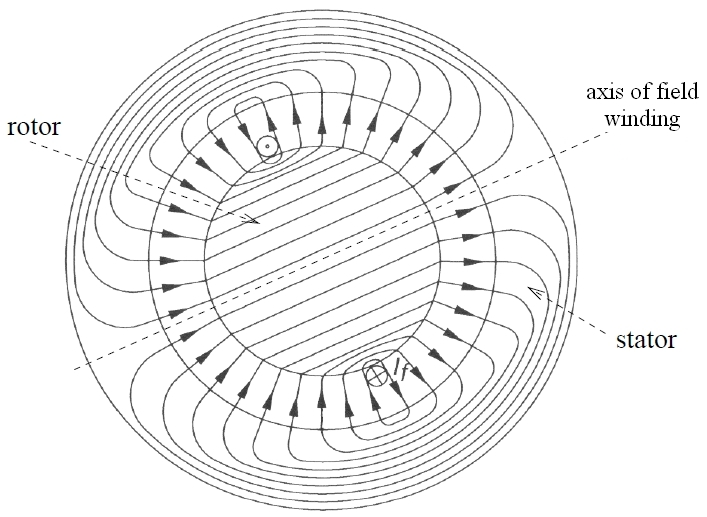
\includegraphics[width=0.92\linewidth,height=0.62\textheight,keepaspectratio]{images/rotor_field.jpg}}
    \end{column}
    \begin{column}{0.48\textwidth}
      \centering
      \textbf{\textcolor{myBlue}{New TikZ Figure (Vector)}}\\[4pt]
      \resizebox{0.92\linewidth}{!}{\providecolor{myRed}{RGB}{209,34,57}
\providecolor{myBlue}{RGB}{28,90,160}
\providecolor{myGreen}{RGB}{34,139,34}
\providecolor{myOrange}{RGB}{210,105,15}
\providecolor{statorIron}{RGB}{234,240,248}
\providecolor{rotorIron}{RGB}{246,247,250}
\providecolor{airGapCol}{RGB}{255,255,255}
\providecolor{fluxCol}{RGB}{20,80,165}

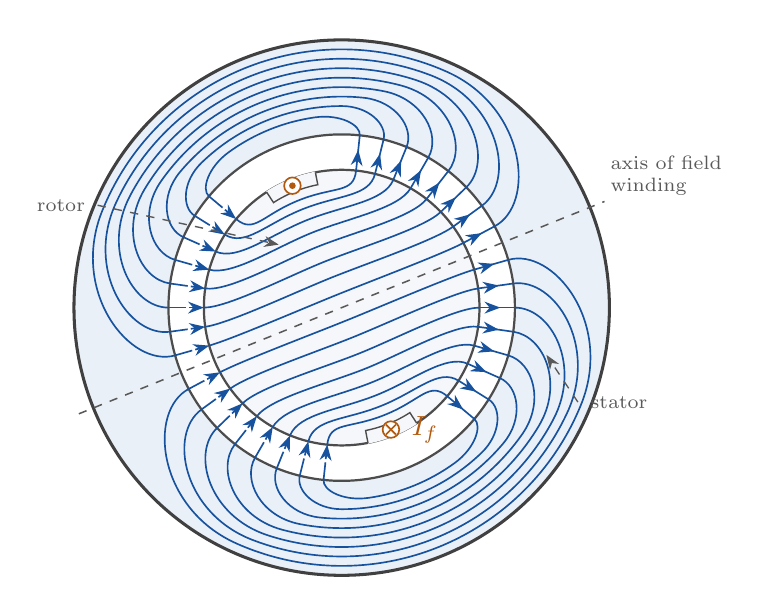
\begin{tikzpicture}[scale=1, >=Stealth, font=\small]

  % Geometry parameters
  \def\Rrotor{1.75}
  \def\Rgap{2.20}
  \def\Rstator{3.40}
  \def\tilt{22} % tilt angle of field winding axis in degrees

  % 1. Iron Cores
  \fill[statorIron] (0,0) circle (\Rstator);
  \fill[airGapCol] (0,0) circle (\Rgap);
  \fill[rotorIron] (0,0) circle (\Rrotor);

  % Boundaries
  \draw[line width=1.1pt, black!75] (0,0) circle (\Rstator);
  \draw[line width=0.8pt, black!70] (0,0) circle (\Rgap);
  \draw[line width=0.8pt, black!70] (0,0) circle (\Rrotor);

  % 2. Magnetic Flux Lines
  % 8 symmetrical loops on each side:
  % dAng: air gap angle from tilt axis
  % Ri: stator yoke radius
  % dPhi: half-span of concentric circular arc centered at tilt+90
  \foreach \dAng/\Ri/\dPhi in {
    6/3.28/46,
    14/3.16/43,
    22/3.04/40,
    30/2.92/37,
    38/2.80/33,
    46/2.68/28,
    54/2.56/22,
    62/2.44/14
  } {
    \pgfmathsetmacro{\angNU}{\tilt + \dAng}
    \pgfmathsetmacro{\angSU}{\tilt + 180 - \dAng}
    \pgfmathsetmacro{\angNL}{\tilt - \dAng}
    \pgfmathsetmacro{\angSL}{\tilt + 180 + \dAng}

    % Upper circuit:
    % 1. Radial air gap transitions with arrows (strictly perpendicular to iron surfaces)
    \draw[line width=0.6pt, fluxCol, ->] (\angNU:\Rrotor) -- (\angNU:{(\Rrotor+\Rgap)/2 + 0.04});
    \draw[line width=0.6pt, fluxCol] (\angNU:{(\Rrotor+\Rgap)/2}) -- (\angNU:\Rgap);

    \draw[line width=0.6pt, fluxCol, <-] (\angSU:\Rrotor) -- (\angSU:{(\Rrotor+\Rgap)/2 - 0.04});
    \draw[line width=0.6pt, fluxCol] (\angSU:{(\Rrotor+\Rgap)/2}) -- (\angSU:\Rgap);

    % 2. Rotor core: smooth flow aligned with tilt axis, curving smoothly to radial at boundary
    \pgfmathsetmacro{\dPerp}{\Rrotor * sin(\dAng) * 0.95}

    \draw[line width=0.6pt, fluxCol]
      (\angSU:\Rrotor) .. controls ($(\angSU:\Rrotor) + ({\tilt-\dAng}:0.3)$) and ($({\tilt+90}:\dPerp) + ({\tilt+180}:0.5)$) .. ($({\tilt+90}:\dPerp)$)
      .. controls ($({\tilt+90}:\dPerp) + (\tilt:0.5)$) and ($(\angNU:\Rrotor) + ({\tilt+180+\dAng}:0.3)$) .. (\angNU:\Rrotor);

    % 3. Upper stator yoke: true concentric circular arc of radius Ri
    \pgfmathsetmacro{\phiStartU}{\tilt + 90 - \dPhi}
    \pgfmathsetmacro{\phiEndU}{\tilt + 90 + \dPhi}
    \coordinate (ArcStartU) at (\phiStartU:\Ri);
    \coordinate (ArcEndU)   at (\phiEndU:\Ri);

    \pgfmathsetmacro{\filletL}{(\Ri - \Rgap) * 0.55}
    \pgfmathsetmacro{\filletTU}{\Ri * sin(\phiStartU - \angNU) * 0.55}

    \draw[line width=0.6pt, fluxCol]
      (\angNU:\Rgap) .. controls ($(\angNU:\Rgap) + (\angNU:\filletL)$) and ($(ArcStartU) + ({\phiStartU-90}:\filletTU)$) .. (ArcStartU)
      arc[start angle=\phiStartU, end angle=\phiEndU, radius=\Ri]
      .. controls ($(ArcEndU) + ({\phiEndU+90}:\filletTU)$) and ($(\angSU:\Rgap) + (\angSU:\filletL)$) .. (\angSU:\Rgap);

    % Lower circuit:
    % 1. Radial air gap transitions with arrows
    \draw[line width=0.6pt, fluxCol, ->] (\angNL:\Rrotor) -- (\angNL:{(\Rrotor+\Rgap)/2 + 0.04});
    \draw[line width=0.6pt, fluxCol] (\angNL:{(\Rrotor+\Rgap)/2}) -- (\angNL:\Rgap);

    \draw[line width=0.6pt, fluxCol, <-] (\angSL:\Rrotor) -- (\angSL:{(\Rrotor+\Rgap)/2 - 0.04});
    \draw[line width=0.6pt, fluxCol] (\angSL:{(\Rrotor+\Rgap)/2}) -- (\angSL:\Rgap);

    % 2. Lower rotor core flow
    \draw[line width=0.6pt, fluxCol]
      (\angSL:\Rrotor) .. controls ($(\angSL:\Rrotor) + ({\tilt+\dAng}:0.3)$) and ($({\tilt-90}:\dPerp) + ({\tilt+180}:0.5)$) .. ($({\tilt-90}:\dPerp)$)
      .. controls ($({\tilt-90}:\dPerp) + (\tilt:0.5)$) and ($(\angNL:\Rrotor) + ({\tilt+180-\dAng}:0.3)$) .. (\angNL:\Rrotor);

    % 3. Lower stator yoke: true concentric circular arc of radius Ri
    \pgfmathsetmacro{\phiStartL}{\tilt - 90 + \dPhi}
    \pgfmathsetmacro{\phiEndL}{\tilt - 90 - \dPhi}
    \coordinate (ArcStartL) at (\phiStartL:\Ri);
    \coordinate (ArcEndL)   at (\phiEndL:\Ri);

    \draw[line width=0.6pt, fluxCol]
      (\angNL:\Rgap) .. controls ($(\angNL:\Rgap) + (\angNL:\filletL)$) and ($(ArcStartL) + ({\phiStartL+90}:\filletTU)$) .. (ArcStartL)
      arc[start angle=\phiStartL, end angle=\phiEndL, radius=\Ri]
      .. controls ($(ArcEndL) + ({\phiEndL-90}:\filletTU)$) and ($(\angSL:\Rgap) + (\angSL:\filletL)$) .. (\angSL:\Rgap);
  }

  % 3. Rotor Field Winding Slots
  % Top slot at tilt + 90 = 112 deg (dot: current out of page)
  \fill[rotorIron] ({\tilt+79}:{\Rrotor+0.01}) 
    -- ({\tilt+79}:{\Rrotor-0.16}) 
    arc[start angle={\tilt+79}, end angle={\tilt+101}, radius={\Rrotor-0.16}] 
    -- ({\tilt+101}:{\Rrotor+0.01}) 
    arc[start angle={\tilt+101}, end angle={\tilt+79}, radius={\Rrotor+0.01}] -- cycle;
  \draw[line width=0.5pt, black!70] ({\tilt+79}:{\Rrotor}) 
    -- ({\tilt+79}:{\Rrotor-0.16}) 
    arc[start angle={\tilt+79}, end angle={\tilt+101}, radius={\Rrotor-0.16}] 
    -- ({\tilt+101}:{\Rrotor});

  \coordinate (SlotTop) at ({\tilt+90}:{\Rrotor-0.08});
  \fill[white] (SlotTop) circle (3.0pt);
  \draw[line width=0.6pt, myOrange!85!black] (SlotTop) circle (3.0pt);
  \fill[myOrange!85!black] (SlotTop) circle (1.2pt);

  % Bottom slot at tilt - 90 = -68 deg (cross: current into page)
  \fill[rotorIron] ({\tilt-79}:{\Rrotor+0.01}) 
    -- ({\tilt-79}:{\Rrotor-0.16}) 
    arc[start angle={\tilt-79}, end angle={\tilt-101}, radius={\Rrotor-0.16}] 
    -- ({\tilt-101}:{\Rrotor+0.01}) 
    arc[start angle={\tilt-101}, end angle={\tilt-79}, radius={\Rrotor+0.01}] -- cycle;
  \draw[line width=0.5pt, black!70] ({\tilt-79}:{\Rrotor}) 
    -- ({\tilt-79}:{\Rrotor-0.16}) 
    arc[start angle={\tilt-79}, end angle={\tilt-101}, radius={\Rrotor-0.16}] 
    -- ({\tilt-101}:{\Rrotor});

  \coordinate (SlotBot) at ({\tilt-90}:{\Rrotor-0.08});
  \fill[white] (SlotBot) circle (3.0pt);
  \draw[line width=0.6pt, myOrange!85!black] (SlotBot) circle (3.0pt);
  \draw[line width=0.6pt, myOrange!85!black] ($(SlotBot)+(-1.8pt,-1.8pt)$) -- ($(SlotBot)+(1.8pt,1.8pt)$);
  \draw[line width=0.6pt, myOrange!85!black] ($(SlotBot)+(-1.8pt,1.8pt)$) -- ($(SlotBot)+(1.8pt,-1.8pt)$);
  \node[right=4pt, font=\normalsize\bfseries, text=myOrange!85!black] at (SlotBot) {$I_f$};

  % 4. Axis of field winding
  \draw[dashed, line width=0.55pt, black!65] ({\tilt+180}:3.6) -- (\tilt:3.6)
    node[above right=-2pt, font=\scriptsize, align=left] {axis of field\\winding};

  % 5. Labels & Pointers
  \draw[dashed, line width=0.5pt, black!65, ->] (-3.1, 1.3) node[left=1pt, font=\scriptsize] {rotor} -- (-0.8, 0.8);
  \draw[dashed, line width=0.5pt, black!65, ->] (3.0, -1.2) node[right=1pt, font=\scriptsize] {stator} -- (2.6, -0.6);

\end{tikzpicture}
}
    \end{column}
  \end{columns}
\end{frame}

% ----------------------------------------------------
% Slide 9 Comparison
% ----------------------------------------------------
\begin{frame}{Slide 9: Field interaction and electromechanical conversion}
  \begin{columns}[c]
    \begin{column}{0.48\textwidth}
      \centering
      \textbf{\textcolor{black!70}{Original Picture (Raster)}}\\[4pt]
      \fbox{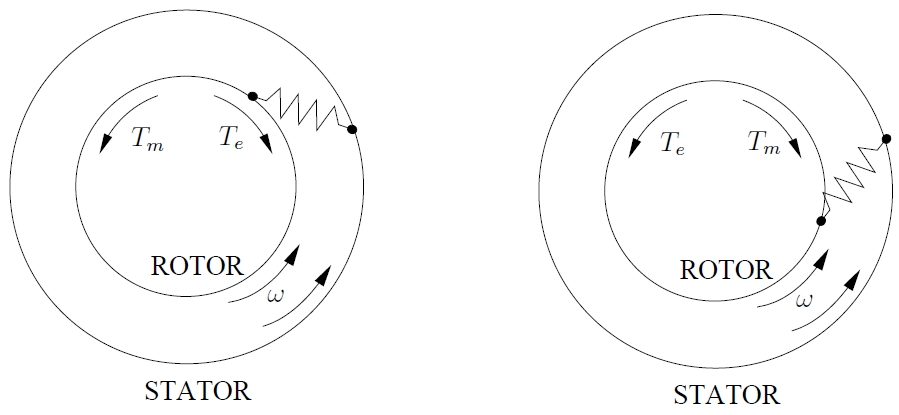
\includegraphics[width=0.95\linewidth,height=0.55\textheight,keepaspectratio]{images/interaction_fields.jpg}}
    \end{column}
    \begin{column}{0.48\textwidth}
      \centering
      \textbf{\textcolor{myBlue}{New TikZ Figure (Vector)}}\\[4pt]
      \resizebox{0.98\linewidth}{!}{\providecolor{myRed}{RGB}{209,34,57}
\providecolor{myBlue}{RGB}{28,90,160}
\providecolor{myGreen}{RGB}{34,139,34}
\providecolor{myOrange}{RGB}{210,105,15}
\providecolor{statorIron}{RGB}{234,240,248}
\providecolor{rotorIron}{RGB}{246,247,250}
\providecolor{airGapCol}{RGB}{255,255,255}

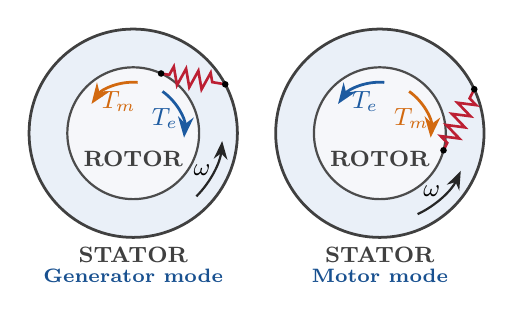
\begin{tikzpicture}[scale=0.54, >=Stealth, font=\small]

  \def\Rrot{1.55}
  \def\Rstat{2.45}

  % ====================================================
  % PANEL (a): GENERATOR MODE
  % ====================================================
  \begin{scope}[shift={(0,0)}]
    % Iron cores
    \fill[statorIron] (0,0) circle (\Rstat);
    \fill[airGapCol] (0,0) circle (\Rrot);
    \fill[rotorIron] (0,0) circle (\Rrot);

    % Boundaries
    \draw[line width=1.0pt, black!75] (0,0) circle (\Rstat);
    \draw[line width=0.8pt, black!70] (0,0) circle (\Rrot);

    % Labels
    \node[font=\footnotesize\bfseries, text=black!75] at (0, -0.6) {ROTOR};
    \node[font=\footnotesize\bfseries, text=black!75] at (0, -2.85) {STATOR};
    \node[font=\scriptsize\bfseries, text=myBlue!90!black] at (0, -3.35) {Generator mode};

    % Speed of rotation omega (counterclockwise in air gap)
    \draw[->, line width=0.8pt, black!85] (-45:{\Rrot+0.55}) arc[start angle=-45, end angle=-5, radius={\Rrot+0.55}];
    %\draw[line width=0.5pt, black!50] (-50:{\Rrot+0.25}) arc[start angle=-50, end angle=-15, radius={\Rrot+0.25}];
    \node[font=\small] at (-28:{\Rrot+0.28}) {$\omega$};

    % Spring: connects Rotor dot at 65 deg to Stator dot at 28 deg
    % Rotor is ahead of Stator!
    \coordinate (RotPtG) at (65:\Rrot);
    \coordinate (StatPtG) at (28:\Rstat);

    \draw[line width=0.95pt, myRed!90!black,
          decorate, decoration={zigzag, segment length=4.5pt, amplitude=3.2pt, pre length=3pt, post length=3pt}]
      (RotPtG) -- (StatPtG);

    \fill[black] (RotPtG) circle (2.2pt);
    \fill[black] (StatPtG) circle (2.2pt);

    % Torques on Rotor:
    % Tm (driving forward CCW)
    \draw[->, line width=1.0pt, myOrange] (85:{\Rrot-0.35}) arc[start angle=85, end angle=145, radius={\Rrot-0.35}];
    \node[font=\small\bfseries, text=myOrange] at (115:{\Rrot-0.73}) {$T_m$};

    % Te (electromagnetic resisting CW)
    \draw[->, line width=1.0pt, myBlue] (55:{\Rrot-0.35}) arc[start angle=55, end angle=-5, radius={\Rrot-0.35}];
    \node[font=\small\bfseries, text=myBlue] at (25:{\Rrot-0.73}) {$T_e$};
  \end{scope}

  % ====================================================
  % PANEL (b): MOTOR MODE
  % ====================================================
  \begin{scope}[shift={(5.8,0)}]
    % Iron cores
    \fill[statorIron] (0,0) circle (\Rstat);
    \fill[airGapCol] (0,0) circle (\Rrot);
    \fill[rotorIron] (0,0) circle (\Rrot);

    % Boundaries
    \draw[line width=1.0pt, black!75] (0,0) circle (\Rstat);
    \draw[line width=0.8pt, black!70] (0,0) circle (\Rrot);

    % Labels
    \node[font=\footnotesize\bfseries, text=black!75] at (0, -0.6) {ROTOR};
    \node[font=\footnotesize\bfseries, text=black!75] at (0, -2.85) {STATOR};
    \node[font=\scriptsize\bfseries, text=myBlue!90!black] at (0, -3.35) {Motor mode};

    % Speed of rotation omega (counterclockwise in air gap)
    \draw[->, line width=0.8pt, black!85] (-65:{\Rrot+0.55}) arc[start angle=-65, end angle=-25, radius={\Rrot+0.55}];
    %\draw[line width=0.5pt, black!50] (-70:{\Rrot+0.25}) arc[start angle=-70, end angle=-35, radius={\Rrot+0.25}];
    \node[font=\small] at (-48:{\Rrot+0.28}) {$\omega$};

    % Spring: connects Rotor dot at -15 deg to Stator dot at 25 deg
    % Stator is ahead of Rotor!
    \coordinate (RotPtM) at (-15:\Rrot);
    \coordinate (StatPtM) at (25:\Rstat);

    \draw[line width=0.95pt, myRed!90!black,
          decorate, decoration={zigzag, segment length=4.5pt, amplitude=3.2pt, pre length=3pt, post length=3pt}]
      (RotPtM) -- (StatPtM);

    \fill[black] (RotPtM) circle (2.2pt);
    \fill[black] (StatPtM) circle (2.2pt);

    % Torques on Rotor:
    % Te (driving forward CCW)
    \draw[->, line width=1.0pt, myBlue] (85:{\Rrot-0.35}) arc[start angle=85, end angle=145, radius={\Rrot-0.35}];
    \node[font=\small\bfseries, text=myBlue] at (115:{\Rrot-0.73}) {$T_e$};

    % Tm (mechanical load resisting CW)
    \draw[->, line width=1.0pt, myOrange] (55:{\Rrot-0.35}) arc[start angle=55, end angle=-5, radius={\Rrot-0.35}];
    \node[font=\small\bfseries, text=myOrange] at (25:{\Rrot-0.73}) {$T_m$};
  \end{scope}

\end{tikzpicture}
}
    \end{column}
  \end{columns}
\end{frame}

% ----------------------------------------------------
% Slide 10 Comparison
% ----------------------------------------------------
\begin{frame}{Slide 10: Salient-pole machine ($p=2$, 4 poles)}
  \begin{columns}[c]
    \begin{column}{0.48\textwidth}
      \centering
      \textbf{\textcolor{black!70}{Original Picture (Raster)}}\\[4pt]
      \fbox{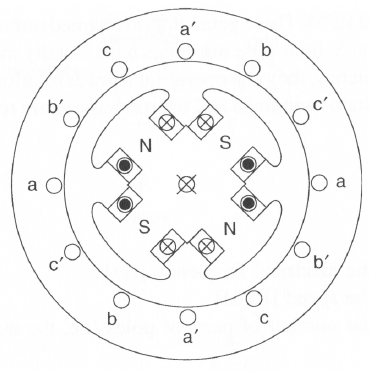
\includegraphics[width=0.92\linewidth,height=0.62\textheight,keepaspectratio]{images/several_poles.jpg}}
    \end{column}
    \begin{column}{0.48\textwidth}
      \centering
      \textbf{\textcolor{myBlue}{New TikZ Figure (Vector)}}\\[4pt]
      \resizebox{0.88\linewidth}{!}{\providecolor{myRed}{RGB}{209,34,57}
\providecolor{myBlue}{RGB}{28,90,160}
\providecolor{myGreen}{RGB}{34,139,34}
\providecolor{myOrange}{RGB}{210,105,15}
\providecolor{statorIron}{RGB}{234,240,248}
\providecolor{rotorIron}{RGB}{246,247,250}
\providecolor{airGapCol}{RGB}{255,255,255}

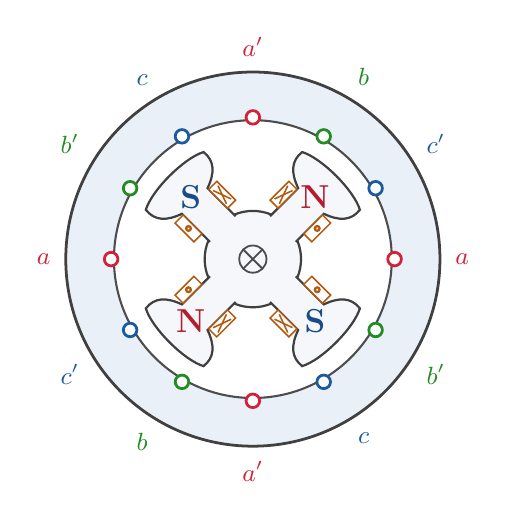
\begin{tikzpicture}[scale=0.72, >=Stealth, font=\small]

  \def\RstatOut{3.30}
  \def\RstatIn{2.45}

  % 1. Stator Iron Core
  \fill[statorIron] (0,0) circle (\RstatOut);
  \fill[airGapCol] (0,0) circle (\RstatIn);
  \draw[line width=1.0pt, black!75] (0,0) circle (\RstatOut);
  \draw[line width=0.75pt, black!70] (0,0) circle (\RstatIn);

  % 2. Rotor Hub
  \fill[rotorIron] (0,0) circle (0.85);

  % Salient Poles (4 poles at 45, 135, 225, 315 deg)
  \foreach \p in {45, 135, 225, 315} {
    \begin{scope}[rotate=\p]
      \fill[rotorIron] 
        (-0.32, 0.75) -- (-0.32, 1.45) 
        .. controls (-0.60, 1.55) and (-0.75, 1.70) .. (-0.72, 1.95)
        .. controls (-0.40, 2.12) and (0.40, 2.12) .. (0.72, 1.95)
        .. controls (0.75, 1.70) and (0.60, 1.55) .. (0.32, 1.45)
        -- (0.32, 0.75) -- cycle;

      \draw[line width=0.8pt, black!75]
        (-0.32, 0.75) -- (-0.32, 1.45) 
        .. controls (-0.60, 1.55) and (-0.75, 1.70) .. (-0.72, 1.95)
        .. controls (-0.40, 2.12) and (0.40, 2.12) .. (0.72, 1.95)
        .. controls (0.75, 1.70) and (0.60, 1.55) .. (0.32, 1.45)
        -- (0.32, 0.75);
    \end{scope}
  }

  % Hub boundary curves between poles
  \foreach \p in {45, 135, 225, 315} {
    \draw[line width=0.8pt, black!75] ({\p+22}:0.85) arc[start angle={\p+22}, end angle={\p+90-22}, radius=0.85];
  }

  % 3. Concentrated Field Coils & Polarity Labels
  % Pole N at 135 deg:
  \begin{scope}[rotate=135]
    % Right coil (cross)
    \draw[line width=0.55pt, myOrange!85!black, fill=white] (-0.52, 0.95) rectangle (-0.32, 1.42);
    \draw[line width=0.55pt, myOrange!85!black] (-0.48, 1.02) -- (-0.36, 1.35);
    \draw[line width=0.55pt, myOrange!85!black] (-0.48, 1.35) -- (-0.36, 1.02);
    
    % Left coil (dot)
    \draw[line width=0.55pt, myOrange!85!black, fill=white] (0.32, 0.95) rectangle (0.52, 1.42);
    \fill[myOrange!85!black] (0.42, 1.185) circle (1.8pt);
    \fill[white] (0.42, 1.185) circle (0.6pt);

    \node[font=\large\bfseries, text=myRed!85!black] at (0, 1.55) {N};
  \end{scope}

  % Pole S at 45 deg:
  \begin{scope}[rotate=45]
    % Right coil (dot)
    \draw[line width=0.55pt, myOrange!85!black, fill=white] (-0.52, 0.95) rectangle (-0.32, 1.42);
    \fill[myOrange!85!black] (-0.42, 1.185) circle (1.8pt);
    \fill[white] (-0.42, 1.185) circle (0.6pt);

    % Left coil (cross)
    \draw[line width=0.55pt, myOrange!85!black, fill=white] (0.32, 0.95) rectangle (0.52, 1.42);
    \draw[line width=0.55pt, myOrange!85!black] (0.36, 1.02) -- (0.48, 1.35);
    \draw[line width=0.55pt, myOrange!85!black] (0.36, 1.35) -- (0.48, 1.02);

    \node[font=\large\bfseries, text=myBlue!85!black] at (0, 1.55) {S};
  \end{scope}

  % Pole S at 225 deg:
  \begin{scope}[rotate=225]
    % Right coil (dot)
    \draw[line width=0.55pt, myOrange!85!black, fill=white] (-0.52, 0.95) rectangle (-0.32, 1.42);
    \fill[myOrange!85!black] (-0.42, 1.185) circle (1.8pt);
    \fill[white] (-0.42, 1.185) circle (0.6pt);

    % Left coil (cross)
    \draw[line width=0.55pt, myOrange!85!black, fill=white] (0.32, 0.95) rectangle (0.52, 1.42);
    \draw[line width=0.55pt, myOrange!85!black] (0.36, 1.02) -- (0.48, 1.35);
    \draw[line width=0.55pt, myOrange!85!black] (0.36, 1.35) -- (0.48, 1.02);

    \node[font=\large\bfseries, text=myBlue!85!black] at (0, 1.55) {S};
  \end{scope}

  % Pole N at 315 deg:
  \begin{scope}[rotate=315]
    % Right coil (cross)
    \draw[line width=0.55pt, myOrange!85!black, fill=white] (-0.52, 0.95) rectangle (-0.32, 1.42);
    \draw[line width=0.55pt, myOrange!85!black] (-0.48, 1.02) -- (-0.36, 1.35);
    \draw[line width=0.55pt, myOrange!85!black] (-0.48, 1.35) -- (-0.36, 1.02);

    % Left coil (dot)
    \draw[line width=0.55pt, myOrange!85!black, fill=white] (0.32, 0.95) rectangle (0.52, 1.42);
    \fill[myOrange!85!black] (0.42, 1.185) circle (1.8pt);
    \fill[white] (0.42, 1.185) circle (0.6pt);

    \node[font=\large\bfseries, text=myRed!85!black] at (0, 1.55) {N};
  \end{scope}

  % 4. Center Shaft
  \draw[line width=0.65pt, black!70] (0,0) circle (0.24);
  \draw[line width=0.65pt, black!70] (-0.17,-0.17) -- (0.17,0.17);
  \draw[line width=0.65pt, black!70] (-0.17,0.17) -- (0.17,-0.17);

  % 5. Stator 12 Conductors (Color-coded by phase)
  % Phase a (Red): 0 (a), 90 (a'), 180 (a), 270 (a')
  \coordinate (C_a0) at (0:{\RstatIn+0.05});
  \fill[white] (C_a0) circle (3.4pt);
  \draw[line width=1.0pt, myRed] (C_a0) circle (3.4pt);
  \node[right=2pt, font=\small\bfseries, text=myRed] at (0:\RstatOut) {$a$};

  \coordinate (C_ap90) at (90:{\RstatIn+0.05});
  \fill[white] (C_ap90) circle (3.4pt);
  \draw[line width=1.0pt, myRed] (C_ap90) circle (3.4pt);
  \node[above=2pt, font=\small\bfseries, text=myRed] at (90:\RstatOut) {$a'$};

  \coordinate (C_a180) at (180:{\RstatIn+0.05});
  \fill[white] (C_a180) circle (3.4pt);
  \draw[line width=1.0pt, myRed] (C_a180) circle (3.4pt);
  \node[left=2pt, font=\small\bfseries, text=myRed] at (180:\RstatOut) {$a$};

  \coordinate (C_ap270) at (270:{\RstatIn+0.05});
  \fill[white] (C_ap270) circle (3.4pt);
  \draw[line width=1.0pt, myRed] (C_ap270) circle (3.4pt);
  \node[below=2pt, font=\small\bfseries, text=myRed] at (270:\RstatOut) {$a'$};

  % Phase b (Green): 60 (b), 150 (b'), 240 (b), 330 (b')
  \coordinate (C_b60) at (60:{\RstatIn+0.05});
  \fill[white] (C_b60) circle (3.4pt);
  \draw[line width=1.0pt, myGreen] (C_b60) circle (3.4pt);
  \node[above right=1pt, font=\small\bfseries, text=myGreen] at (60:\RstatOut) {$b$};

  \coordinate (C_bp150) at (150:{\RstatIn+0.05});
  \fill[white] (C_bp150) circle (3.4pt);
  \draw[line width=1.0pt, myGreen] (C_bp150) circle (3.4pt);
  \node[above left=1pt, font=\small\bfseries, text=myGreen] at (150:\RstatOut) {$b'$};

  \coordinate (C_b240) at (240:{\RstatIn+0.05});
  \fill[white] (C_b240) circle (3.4pt);
  \draw[line width=1.0pt, myGreen] (C_b240) circle (3.4pt);
  \node[below left=1pt, font=\small\bfseries, text=myGreen] at (240:\RstatOut) {$b$};

  \coordinate (C_bp330) at (330:{\RstatIn+0.05});
  \fill[white] (C_bp330) circle (3.4pt);
  \draw[line width=1.0pt, myGreen] (C_bp330) circle (3.4pt);
  \node[below right=1pt, font=\small\bfseries, text=myGreen] at (330:\RstatOut) {$b'$};

  % Phase c (Blue): 30 (c'), 120 (c), 210 (c'), 300 (c)
  \coordinate (C_cp30) at (30:{\RstatIn+0.05});
  \fill[white] (C_cp30) circle (3.4pt);
  \draw[line width=1.0pt, myBlue] (C_cp30) circle (3.4pt);
  \node[above right=1pt, font=\small\bfseries, text=myBlue] at (30:\RstatOut) {$c'$};

  \coordinate (C_c120) at (120:{\RstatIn+0.05});
  \fill[white] (C_c120) circle (3.4pt);
  \draw[line width=1.0pt, myBlue] (C_c120) circle (3.4pt);
  \node[above left=1pt, font=\small\bfseries, text=myBlue] at (120:\RstatOut) {$c$};

  \coordinate (C_cp210) at (210:{\RstatIn+0.05});
  \fill[white] (C_cp210) circle (3.4pt);
  \draw[line width=1.0pt, myBlue] (C_cp210) circle (3.4pt);
  \node[below left=1pt, font=\small\bfseries, text=myBlue] at (210:\RstatOut) {$c'$};

  \coordinate (C_c300) at (300:{\RstatIn+0.05});
  \fill[white] (C_c300) circle (3.4pt);
  \draw[line width=1.0pt, myBlue] (C_c300) circle (3.4pt);
  \node[below right=1pt, font=\small\bfseries, text=myBlue] at (300:\RstatOut) {$c$};

\end{tikzpicture}
}
    \end{column}
  \end{columns}
\end{frame}

\end{document}
